\documentclass[conference]{IEEEtran}
\IEEEoverridecommandlockouts

% -----------------------------------------------------------------------------
% PACKAGES
% -----------------------------------------------------------------------------
\usepackage{amsmath,amssymb,amsfonts}
\usepackage{graphicx}
\usepackage{textcomp}
\usepackage{xcolor}
\usepackage{booktabs}
\usepackage{cite}
\usepackage{url}
\usepackage{microtype}
\usepackage{tikz}
\usetikzlibrary{arrows.meta,positioning,calc,shapes.geometric}
\usepackage{pgfplots}
\pgfplotsset{compat=1.16}
\usepgfplotslibrary{fillbetween}
\usepackage[hidelinks]{hyperref}

% Common style for every plot
\pgfplotsset{
  every axis/.append style={
    font=\scriptsize,
    tick label style={font=\tiny},
    label style={font=\scriptsize},
    title style={font=\footnotesize\bfseries, yshift=-2pt},
    grid=both, grid style={dotted, black!20},
    legend style={font=\tiny, draw=black!30, fill=white, fill opacity=0.85, text opacity=1},
  }
}

\hyphenation{op-tical net-works semi-conduc-tor multi-modal}

\begin{document}

% -----------------------------------------------------------------------------
% TITLE & AUTHORS
% -----------------------------------------------------------------------------
\title{When Scale Silences a Modality: Disentangling Representation Magnitude, Optimization Dynamics, and Evaluation Artifacts in Multimodal Collapse}
\author{
\begin{tabular}[t]{@{}c@{}}
  Komal Lamba\\[2pt]
  \textit{School of Computing and Artificial Intelligence}\\
  \textit{Lovely Professional University}\\
  Phagwara, Punjab, India\\
  lamba6765@gmail.com
\end{tabular}
\hspace{1.2cm}
\begin{tabular}[t]{@{}c@{}}
  Ankita Maji\\[2pt]
  \textit{School of Computing and Artificial Intelligence}\\
  \textit{Lovely Professional University}\\
  Phagwara, Punjab, India\\
  ankitamaji7033@gmail.com
\end{tabular}
\\[1.5em]
\begin{tabular}[t]{@{}c@{}}
  Prabhutee Neb\\[2pt]
  \textit{School of Computing and Artificial Intelligence}\\
  \textit{Lovely Professional University}\\
  Phagwara, Punjab, India\\
  nebprabhutee@gmail.com
\end{tabular}
\hspace{1.2cm}
\begin{tabular}[t]{@{}c@{}}
  Premananda Sahu\\[2pt]
  \textit{School of Computer Science and Engineering}\\
  \textit{Lovely Professional University}\\
  Phagwara, Punjab, India\\
  prema.uce@gmail.com
\end{tabular}
}

\maketitle

% -----------------------------------------------------------------------------
% ABSTRACT
% -----------------------------------------------------------------------------
\begin{abstract}
A common failing in multimodal deep learning architectures is what is known as \textit{modality collapse} in which the network is strongly influenced by a single modality while attenuating feature streams of other modalities. Most previous studies have blamed this mismatch on either asynchrony in the learning speeds, or on task-difficulty mismatches, and the \textit{scale hypothesis} has received little attention: does feature-magnitude disparity between the modality encoders directly cause collapse? Furthermore, traditional benchmarking approach uses the naive zero-masking accuracy measure which merges out-of-distribution degradation of classifiers with actual representational error. We empirically show that forward activation scaling ($h_A' = \alpha h_A$) and backward gradient scaling ($\nabla_{\theta_A}\mathcal{L} \leftarrow \alpha \nabla_{\theta_A}\mathcal{L}$) are distinct and then theoretically explain their differences. We use a frozen-encoder linear probe evaluation battery, mean-ablation dominance and Shapley values on a set of 160 controlled synthetic runs, 520 mechanistic runs and on real-world audio-visual emotion recognition (CREMA-D). %
Our conclusions: (1) early activation-norm disparity tracks early dominance (Spearman $r_s = 0.98$ at epoch 5); (2) trainable encoders adaptively compensate over training, shrinking the scale ratio from $[0.14, 7.55]$ to $[0.60, 1.68]$; (3) adaptive optimizers (Adam/AdamW) cancel a constant gradient gain, with $\rho_{\Delta\theta} = 1.001 \pm 0.011$; (4) SGD passes the gain through, with $\rho_{\Delta\theta} = 95.8 \pm 4.6$; and (5) extreme forward scaling measurably harms representations in a low-capacity synthetic regime, whereas on CREMA-D the large zero-masking shift ($\Delta D_{\text{mask}} = +0.259 \pm 0.044$) is not confirmed by decoupled metrics (mean ablation $+0.012$, Shapley $+0.014$, both $p > 0.05$). Feature scale alone therefore does not appear sufficient to cause persistent collapse in converged real-world models, and naive masking is a common source of false-positive diagnoses.
\end{abstract}

\begin{IEEEkeywords}
Multimodal Learning, Modality Collapse, Optimization Dynamics, Adaptive Gradient Methods, Feature Scaling, Shapley Values, Linear Probing.
\end{IEEEkeywords}

% -----------------------------------------------------------------------------
% I. INTRODUCTION
% -----------------------------------------------------------------------------
\section{Introduction}
 \IEEEPARstart{M}{ultimodal} neural networks aim to discover synergy in the representations of heterogeneous data streams by producing a multimodal latent embedding that combines acoustic speech and visual facial dynamics \cite{baltrusaitis2019multimodal}.%
 Effective fusion outperforms any unimodal baseline and this unimodal gain ($G > 0$) is a measure of the effectiveness of fusion. Joint optimization, however, has a lot of competitive dynamics. However, the joint models often experience \textit{modality collapse} or \textit{modality suppression} or \textit{modality dominance}, which is equivalent to degraded into unimodal system \cite{wang2020makes, peng2022balanced, wu2022characterizing}.

\subsection{Background and Motivation}
The main causes suggested in prevailing explanations are discrepancies between the rates of unimodal convergence or inductive biases. In \cite{wang2020makes}, Wang et al. demonstrated that modalities take different amounts of time to converge, and the modality with less convergence dominates the joint loss at the beginning of training. Dynamic rescaling of back-propagated gradients by unimodal loss trajectories is done via mitigation strategies like on-the-fly gradient modulation (OGM-GE) \cite{peng2022balanced} and prototypical modal rebalancing (PMR) \cite{fan2023pmr}.

Nevertheless, a structural question has not been answered: \textit{does feature-magnitude disparity between modalities causally drive modality collapse?} In practice, two different kinds of encoders (e.g., a 1D audio CNN and a 2D visual ResNet) produce embeddings of very different norms ($\|h_A\| \gg \|h_V\|$). An intuitive understanding is that the modality with higher activations is given precedence in the fusion layer, and the lower activations are not provided with any optimization signal.

\subsection{The Evaluation Conundrum}
Nearly all measures of modality dominance are based on \textit{zero-masking}: setting the test-time representations of one modality to zero and measuring the subsequent accuracy loss \cite{wang2020makes, fan2023pmr}. If the model is trained with scale disparity, however, the classification head adjusts to the distribution of numbers that it is receiving. If the distribution deviates from the zero-masking distribution, it will lead to errors due to the misalignment of the classifiers instead of the noise in the encoder representation. The literature can fall into the trap of diagnosing collapse when there is none if there is no decoupled evaluation.

\subsection{Research Questions}
In this work, we answer four research questions:
\begin{itemize}
    \item \textbf{RQ1 (Causal Scale Sufficiency):} Do changes in the magnitude of features alone cause real collapse of representation?
    \item \textbf{RQ2 (Early Diagnostic Validity):} Can an early activation-norm ratio $\rho$ be used to determine the modality dominance prior to convergence?
    \item \textbf{RQ3 (Optimization Disentanglement):} What is the difference between adaptive (Adam/AdamW) and non-adaptive (SGD) optimizers with respect to forward vs gradient scale interventions?
    \item \textbf{RQ4 (Decoupled vs.\ Naive Evaluation):} Are zero-masking metrics a good measure of representational degradation in the presence of linear probes, mean ablation and Shapley values?
\end{itemize}

\subsection{Key Contributions}
\begin{enumerate}
    \item Separating forward scale from gradient scale: an experimental paradigm disentangling forward scale ($h_A' = \alpha h_A$) from backward gradient scale ($\nabla_{\theta_A}\mathcal{L} \leftarrow \alpha \nabla_{\theta_A}\mathcal{L}$), to separate representation magnitude from update intensity.
    \item The ratio $\rho = \mathbb{E}[\|h_A\|] / \mathbb{E}[\|h_V\|]$ is almost perfectly rank-correlated with dominance at epoch 5 ($r_s = 0.98$), while the trainable encoders make up for that performance by converging this ratio, reducing the range from $[0.14, 7.55]$ to $[0.60, 1.68]$.
    \item Adam, when normalized by the second moment, removes gradient disparities, with $\rho_{\Delta\theta} = 1.001 \pm 0.011$; in SGD, rescaling the learning-rate removes the gradient disparities, with $D = +0.003$.
    \item On the real data CREMA-D, the forward collapse is strong with the zero-masking protocol ($\Delta D_{\text{mask}} = +0.259 \pm 0.044$), whereas it is not significantly degraded for probes and Shapley values ($\Delta \text{Probe} = +0.023$; $\Delta \text{Shapley} = +0.014$, $p > 0.05$).
\end{enumerate}

% -----------------------------------------------------------------------------
% II. RELATED WORK
% -----------------------------------------------------------------------------
\section{Related Work}
\textbf{Modality Competition and Optimization Imbalance.}
It was demonstrated by Wang et al.\ \cite{wang2020makes} that the convergence rates of different unimodal networks are often quite different, and therefore joint multimodal networks may not converge to their performance level better than unimodal networks. They suggested to blend the gradients based on the overfitting speeds of the unimodal networks. Peng et al.\ \cite{peng2022balanced} proposed a technique called OGM-GE which reduces the gradient of the faster converging modality. Fan et al.\ \cite{fan2023pmr} proposed PMR, which regularizes the inter-class margins in prototype spaces. Wu et al. \cite{wu2022characterizing} analyzed the negative aspects of fine-tuning for multimodal learning. These all work by changing gradients, assuming that task difficulty or optimization speed is the cause, but then don't investigate directly what effect this has on numerical features' scale.

\textbf{Adaptive Optimization and Scale Invariance.}
Kingma and Ba \cite{kingma2015adam} proposed Adam which rescales the coordinate updates by the square root of exponentially decaying squared-gradient moments; Loshchilov and Hutter \cite{loshchilov2019decoupled} decoupled weight decay in AdamW. Wilson et al.\ \cite{wilson2017marginal} and Zhang et al.\ \cite{zhang2020adaptive} analyzed this difference in generalization between Adam and SGD, and showed that coordinate-wise adaptivity provides scale invariance up to the smoothing parameter $\epsilon$. The interplay between adaptive normalization of the multiple branches of the encoder has not been studied in an explicit yet systematic manner in the context of multimodal settings.

\textbf{Interpretability, Probes and Decoupled Metrics.}
Alain and Bengio \cite{alain2016understanding} proposed linear classifier probes to evaluate the linearly accessible content of the frozen representations. Morcos et al.\ \cite{morcos2018importance} demonstrated that the absence of ablation leads to out-of-distribution artifacts and favored mean ablation. The SHAP values \cite{lundberg2017unified} which allocate predictive credit between coalitions, are popularized with the help of Cooperative game theory, from which we are borrowing the term \cite{shapley1953value}.%
 These tools are integrated into a common multimodal collapse audit protocol.

% -----------------------------------------------------------------------------
% III. PROBLEM FORMULATION
% -----------------------------------------------------------------------------
\section{Problem Formulation}

% FIGURE 1: Comprehensive Architecture and Diagnostic Framework
\begin{figure*}[!t]
\centering
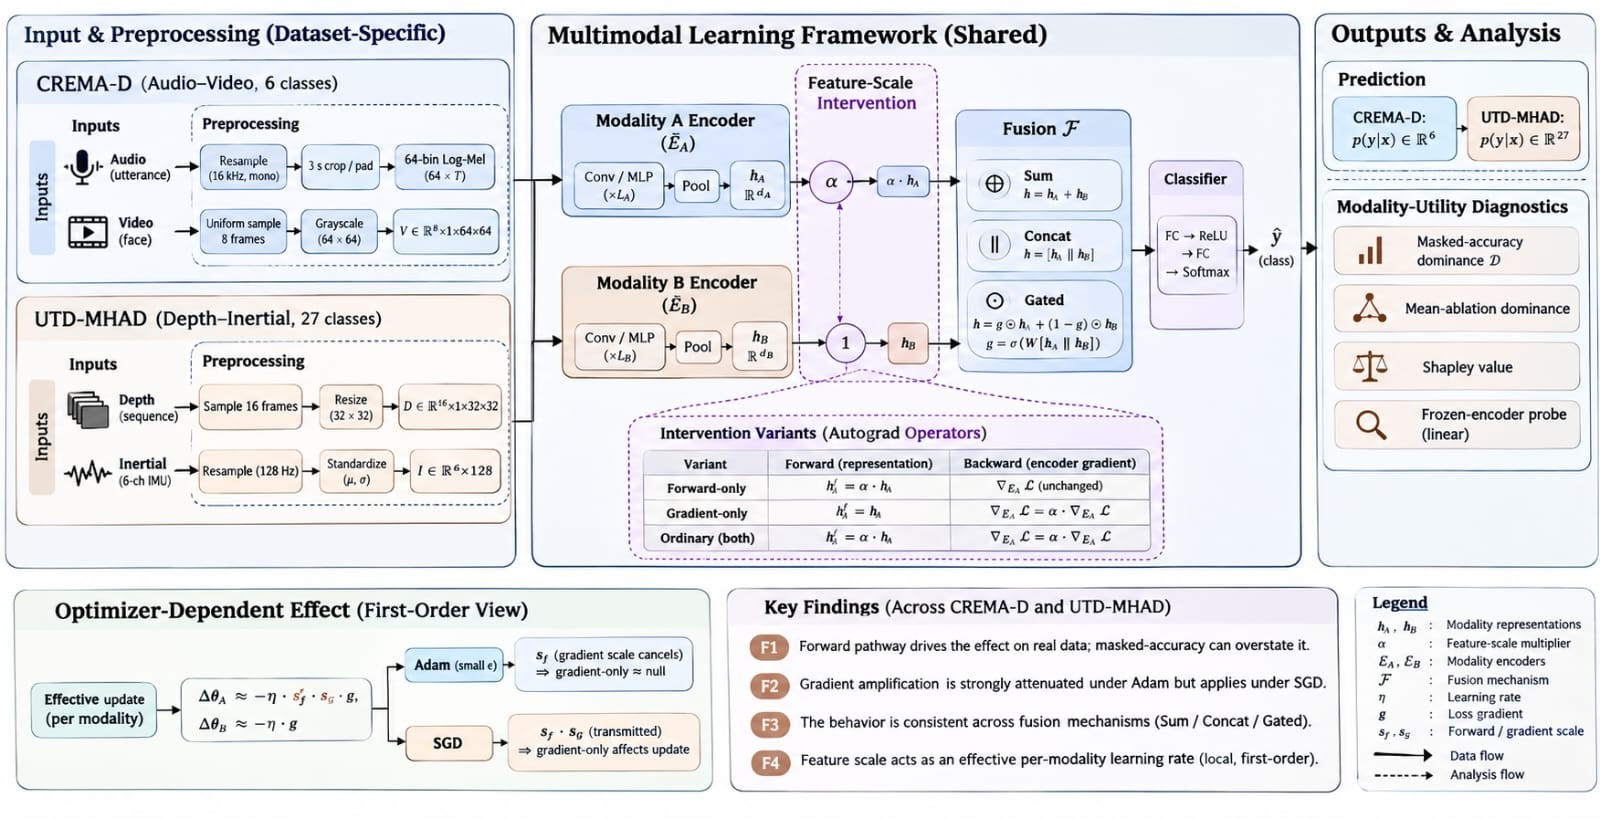
\includegraphics[width=\textwidth]{figures/architecture_diagram.jpg}
\caption{The overview of the scale-investigation framework and diagnostic suite. A dedicated preprocessor, called an encoder, $E_A$ or $E_B$, preprocesses and maps the modality input streams, e.g., audio-video in CREMA-D and depth-inertial in UTD-MHAD, to latent representations $h_A$ or $h_B$. Three variants of Autograd operators are injected: forward-only, gradient-only, ordinary scaling, where features are controlled at the modality $A$ and units at the modality $B$ at feature scale. The classification head receives multimodal fusion $\mathcal{F}$ (Sum, Concat or Gated). The framework combines a multi-metric diagnostic suite (masked dominance $D$, mean ablation, Shapley values $\phi_m$ and frozen linear probes) with first-order optimizer dynamics identifying the difference between Adam second-moment scale cancellation and SGD linear update drift, creating core findings (F1--F4).}
\label{fig:architecture}
\end{figure*}

\subsection{Multimodal Predictive Pipeline}
Suppose that we have a multimodal dataset $\mathcal{D} = \{(x_A^{(i)}, x_V^{(i)}, y^{(i)})\}_{i=1}^N$ consisting of $N$ multimodal samples, with the primary modality $x_A$ (e.g., audio utterance), secondary modality $x_V$ (e.g., visual face dynamics), and label $y \in \{1, \dots, C\}$ to be classified. The raw input is projected to a latent representation by the heterogeneous modality encoders $E_A = f_A(\cdot; \theta_A) \in \mathbb{R}^d$ and $E_B = f_V(\cdot; \theta_V) \in \mathbb{R}^d$. A fusion operator $\Phi$ (sum, concatenation, gated fusion, as shown in Fig.~\ref{fig:architecture}) is then used to combine these representations together into a joint embedding $z = \Phi(h_A, h_V) = \sigma(W_f [h_A; h_V] + b_f) \in \mathbb{R}^D$. The joint network is trained by minimizing the empirical cross-entropy loss $\mathcal{L}(\theta) = -\frac{1}{N} \sum_{i=1}^N \sum_{c=1}^C y_{c}^{(i)} \log \hat{y}_{c}^{(i)}$.

\subsection{Scale Interventions}
We generalize 3 targeted intervention operators functioned by a positive parameter $\alpha$ and formalized them in the Autograd operator table of Fig.~\ref{fig:architecture} as systematized:
\begin{enumerate}
    \item \textbf{Forward-only ($\mathcal{T}_{\text{fwd}}$):} For this type of model, the latent representation of modality $A$ is scaled during inference and forward propagation, such that $h_A' = \alpha \cdot h_A$ with $z = \Phi(h_A', h_V)$, and the encoder gradient, $\nabla_{\theta_A}\mathcal{L}$, is unscaled through back propagation.
    \item \textbf{Gradient-only ($\mathcal{T}_{\text{grad}}$):} The forward pass is unchanged, that is $h_A' = h_A$; however, the backpropagated gradient with respect to the modality-$A$ encoder parameters is scaled by a factor of $\alpha$ while the gradient with respect to the modality-$V$ encoder parameters is left unchanged, that is $\nabla_{\theta_V}\mathcal{L}' = \nabla_{\theta_V}\mathcal{L}$.
    \item \textbf{Ordinary ($\mathcal{T}_{\text{ord}}$):} Scaling is applied to both forward activations and backward gradients ($h_A' = \alpha h_A$ and $\nabla_{\theta_A}\mathcal{L}' = \alpha \nabla_{\theta_A}\mathcal{L}$).
\end{enumerate}

\subsection{Diagnostic and Evaluation Metrics}
Our diagnostic battery (Fig.~\ref{fig:architecture}, top-right) records five complementary metrics to audit representational fidelity without classifier confounding:

\textbf{1) Activation-norm ratio ($\rho$):} directly measured at the fusion boundary:
\begin{equation}
    \rho = \frac{\mathbb{E}_{(x_A, x_V) \sim \mathcal{D}} [\|h_A\|_2]}{\mathbb{E}_{(x_A, x_V) \sim \mathcal{D}} [\|h_V\|_2]}.
    \label{eq:activation_ratio}
\end{equation}
These values in the vicinity of $\rho \approx 1$ indicate moderate magnitudes, while $\rho \gg 1$ indicate that the numerical magnitude of $A$ is significantly larger.

\textbf{2) Parameter update ratio ($\rho_{\Delta\theta}$):} Indicates the relative speed of the parameter trajectory between the two encoders, expressed as $\rho_{\Delta\theta} = \|\theta_A^{(t+1)} - \theta_A^{(t)}\|_2 / \|\theta_V^{(t+1)} - \theta_V^{(t)}\|_2$.

\textbf{3) Modality dominance index ($D$):} The standard-literature index to measure the accuracy loss caused by the zero-masking:
\begin{equation}
    D = \text{Acc}(\text{Model} \mid x_V = \mathbf{0}) - \text{Acc}(\text{Model} \mid x_A = \mathbf{0}),
    \label{eq:dominance_index}
\end{equation}
where $D$ is positive is the case of apparent audio dominance under zero-imputation.

\textbf{4) Decoupled linear probe accuracy ($\text{Acc}_{\text{probe}}$):} Measures the discriminative content of frozen encoder $f_A$ in the linear space, using $\hat{y}_{\text{probe}} = \text{Softmax}(W_{\text{probe}} f_A(x_A; \theta_A^*) + b_{\text{probe}})$, where $W_{\text{probe}}$ is optimized independently of the multimodal run.

\textbf{5) Cooperative Shapley contribution ($\phi_m$):} The marginal utility for coalition $M = \{A, V\}$ is calculated as:
\begin{equation}
    \phi_A = \sum_{S \subseteq M \setminus \{A\}} \frac{|S|!(|M| - |S| - 1)!}{|M|!} [v(S \cup \{A\}) - v(S)],
    \label{eq:shapley}
\end{equation}
Characteristic function $v(S)$ measures the accuracy on the test set over the modalities active on $S$, while each modality excluded from $S$ is replaced by its training-set mean representation (mean ablation).

% -----------------------------------------------------------------------------
% IV. METHODOLOGY
% -----------------------------------------------------------------------------
\section{Methodology and Theoretical Analysis}

% FIGURE 2
\begin{figure*}[!t]
\centering
\resizebox{0.97\textwidth}{!}{%
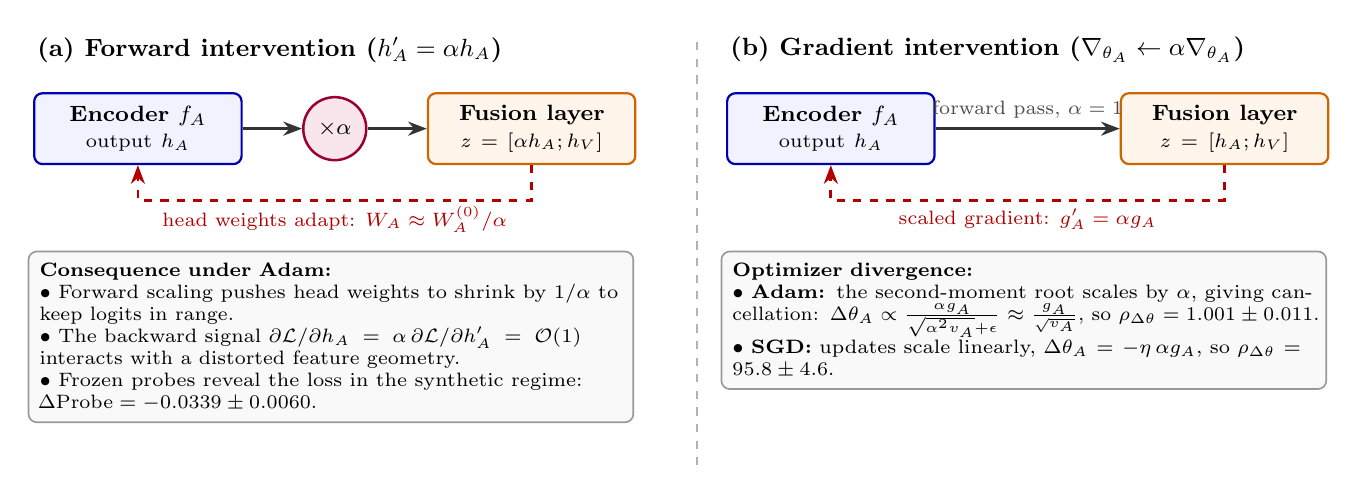
\begin{tikzpicture}[
    nodeBox/.style={rectangle, draw=blue!70!black, fill=blue!5, rounded corners=3pt, text width=2.4cm, minimum height=0.9cm, align=center, font=\footnotesize\bfseries, line width=0.8pt},
    mulCircle/.style={circle, draw=purple!80!black, fill=purple!10, minimum size=0.8cm, align=center, font=\footnotesize\bfseries, line width=0.9pt},
    fuseBox/.style={rectangle, draw=orange!80!black, fill=orange!8, rounded corners=3pt, text width=2.4cm, minimum height=0.9cm, align=center, font=\footnotesize\bfseries, line width=0.8pt},
    noteBox/.style={rectangle, draw=black!40, fill=gray!5, rounded corners=3pt, text width=7.4cm, align=left, font=\scriptsize, line width=0.6pt, inner sep=4pt},
    arrowFwd/.style={-{Stealth[scale=0.9]}, line width=1.0pt, draw=black!80},
    arrowBack/.style={-{Stealth[scale=0.9]}, line width=1.0pt, draw=red!70!black, dashed}
]
    % (a)
    \node[anchor=west, font=\small\bfseries] at (-0.2, 2.7) {(a) Forward intervention ($h_A' = \alpha h_A$)};
    \node[nodeBox] (fa1) at (1.2, 1.7) {Encoder $f_A$\\ \normalfont\scriptsize output $h_A$};
    \node[mulCircle] (mul1) at (3.7, 1.7) {$\times\alpha$};
    \node[fuseBox] (fuse1) at (6.2, 1.7) {Fusion layer\\ \normalfont\scriptsize $z = [\alpha h_A; h_V]$};
    \draw[arrowFwd] (fa1) -- (mul1);
    \draw[arrowFwd] (mul1) -- (fuse1);
    \draw[arrowBack] (fuse1.south) -- ++(0,-0.45) -| (fa1.south);
    \node[font=\scriptsize, color=red!70!black] at (3.7, 0.55) {head weights adapt: $W_A \approx W_A^{(0)}/\alpha$};

    \node[noteBox, anchor=north west] at (-0.2, 0.15) {\textbf{Consequence under Adam:}\\
    $\bullet$ Forward scaling pushes head weights to shrink by $1/\alpha$ to keep logits in range.\\
    $\bullet$ The backward signal $\partial\mathcal{L}/\partial h_A = \alpha\,\partial\mathcal{L}/\partial h_A' = \mathcal{O}(1)$ interacts with a distorted feature geometry.\\
    $\bullet$ Frozen probes reveal the loss in the synthetic regime: $\Delta\text{Probe} = -0.0339 \pm 0.0060$.};%

    \draw[line width=0.6pt, draw=black!30, dashed] (8.3, 2.8) -- (8.3, -2.6);

    % (b)
    \node[anchor=west, font=\small\bfseries] at (8.6, 2.7) {(b) Gradient intervention ($\nabla_{\theta_A} \leftarrow \alpha \nabla_{\theta_A}$)};
    \node[nodeBox] (fa2) at (10.0, 1.7) {Encoder $f_A$\\ \normalfont\scriptsize output $h_A$};
    \node[fuseBox] (fuse2) at (15.0, 1.7) {Fusion layer\\ \normalfont\scriptsize $z = [h_A; h_V]$};
    \draw[arrowFwd] (fa2) -- node[above, font=\scriptsize\color{black!70}] {forward pass, $\alpha = 1$} (fuse2);
    \draw[arrowBack] (fuse2.south) -- ++(0,-0.45) -| (fa2.south);
    \node[font=\scriptsize, color=red!70!black] at (12.5, 0.55) {scaled gradient: $g_A' = \alpha g_A$};

    \node[noteBox, anchor=north west] at (8.6, 0.15) {\textbf{Optimizer divergence:}\\
    $\bullet$ \textbf{Adam:} the second-moment root scales by $\alpha$, giving cancellation: $\Delta\theta_A \propto \frac{\alpha g_A}{\sqrt{\alpha^2 v_A} + \epsilon} \approx \frac{g_A}{\sqrt{v_A}}$, so $\rho_{\Delta\theta} = 1.001 \pm 0.011$.\\
    $\bullet$ \textbf{SGD:} updates scale linearly, $\Delta\theta_A = -\eta\,\alpha g_A$, so $\rho_{\Delta\theta} = 95.8 \pm 4.6$.};%
\end{tikzpicture}}
\caption{Mechanistic comparison of (a) forward intervention, where head adaptation alters representation geometry, and (b) gradient intervention, where Adam's second-moment denominator cancels the gradient scale ($\rho_{\Delta\theta} = 1.001$) while SGD suffers severe parameter drift ($\rho_{\Delta\theta} = 95.8$).}
\label{fig:forward_vs_gradient}
\end{figure*}

\subsection{Overall System Architecture}
Our framework, as shown in Fig.~\ref{fig:architecture}, is end-to-end and systematically couples pre-processing, dual-stream feature encoding, targeted Autograd interventions, and a multi-angle diagnostic battery for the dataset. The first-order optimizer dynamics (Fig.~\ref{fig:architecture} bottom-left) explicitly map how forward and backward scale factors propagate through adaptive versus non-adaptive optimizers, directly establishing our four main results (F1-F4 in Fig.~\ref{fig:architecture}): forward scaling effects change representation geometry and head calibration in all fusion mechanisms, while gradient scaling is strongly dampened by adaptive optimizers.

\subsection{Why Adam and SGD Diverge: Theoretical Analysis}
Adaptive and non-adaptive optimizers react very differently to scale interventions, as shown in Fig.~\ref{fig:forward_vs_gradient} and Fig.~\ref{fig:architecture} (bottom-left).

Suppose that a parameter $w \in \theta_A$ is subjected to a gradient intervention, $\mathcal{T}_{\text{grad}}$, such that the gradient satisfies $g_t' = \alpha g_t$ (gradient scaling). With exponential decay parameters $\beta_1, \beta_2$, the biased moment estimates scale as $m_t' = \beta_1 m_{t-1}' + (1 - \beta_1)(\alpha g_t) = \alpha m_t$ and $v_t' = \beta_2 v_{t-1}' + (1 - \beta_2)(\alpha g_t)^2 = \alpha^2 v_t$. Then the bias-corrected parameter update is calculated as:
\begin{equation}
    \Delta w_t' = -\eta \frac{\hat{m}_t'}{\sqrt{\hat{v}_t'} + \epsilon} = -\eta \frac{\hat{m}_t}{\sqrt{\hat{v}_t} + \epsilon/\alpha} \approx -\eta \frac{\hat{m}_t}{\sqrt{\hat{v}_t}} = \Delta w_t,
    \label{eq:adam_cancellation}
\end{equation}
for all $t$ such that $\alpha \sqrt{\hat{v}_t} \gg \epsilon$. An overall scale factor $\alpha$ is absorbed in the second-moment root, thus ensuring that $\rho_{\Delta\theta} \approx 1$ mathematically.

In stark contrast, the parameter step of SGD with learning rate $\eta$ scales linearly with the gradient multiplier:
\begin{equation}
    \Delta w_t' = -\eta\, g_t' = -\eta\,\alpha\, g_t = \alpha\,\Delta w_t
    \quad\Rightarrow\quad
    \rho_{\Delta\theta}^{(\text{SGD})} \approx \alpha\,\rho_{\Delta\theta}^{(\text{baseline})},
    \label{eq:sgd_drift}
\end{equation}
The same linear dependence remains when the momenta is non-zero $\mu$ as the velocity buffer is a linear filter of the historical gradients. The linear transmission is a direct destabilizing effect of the optimization process unless it is balanced by an inverse per-modality learning rate $\eta_A = \eta / \alpha$.

\subsection{Forward-Scale Degradation}
Adam does not neutralize forward scaling but it does neutralize gradient scaling. When the scaled representation $\alpha h_A$ enters fusion with $\alpha \gg 1$, the classification head quickly shrinks the corresponding weights, $W_{c,A} \approx W_{c,A}^{(0)}/\alpha$, to avoid logit explosion. Thus, the error signal returned to encoder $f_A$ is a back propagated error signal such that:
\begin{equation}
    \frac{\partial \mathcal{L}}{\partial h_A} = \alpha \frac{\partial \mathcal{L}}{\partial h_A'} \approx \alpha \cdot \mathcal{O}\!\left(\frac{1}{\alpha}\right) = \mathcal{O}(1).
    \label{eq:forward_gradient}
\end{equation}
which maintains the magnitude of the gradient (but optimizes across a very compressed and distorted latent geometry) and leads to a measurable decrease in the accuracy of the probes in capacity constrained models.

% -----------------------------------------------------------------------------
% V. EXPERIMENTAL SETUP
% -----------------------------------------------------------------------------
\section{Experimental Setup}

\begin{table}[!t]
\centering
\caption{Experimental Setup and Hyperparameters}
\label{tab:hyperparams}
\renewcommand{\arraystretch}{1.1}
\resizebox{\columnwidth}{!}{%
\begin{tabular}{lll}
\toprule
\textbf{Parameter} & \textbf{Synthetic} & \textbf{CREMA-D} \\
\midrule
Hardware & RTX 4070 Laptop (8.6 GB) & RTX 4070 Laptop (8.6 GB) \\
PyTorch / CUDA & 2.x / 12.x & 2.x / 12.x \\
Random seeds & 10 (5 in the ratio sweep) & 5 \\
Batch size & 256 & 64 \\
Epochs & 40 (early: epoch 5) & 30 \\
Optimizers & Adam, SGD (momentum 0.9) & AdamW (wd 0, i.e.\ Adam), SGD (momentum 0.9) \\
Base learning rate & $10^{-3}$ & $10^{-3}$ (SGD: $3\times10^{-2}$; $10^{-2}$ with clipping) \\
$(\beta_1, \beta_2)$ & (0.9, 0.999) & (0.9, 0.999) \\
Adam $\epsilon$ & $10^{-8}$ (swept to $10^{-2}$) & $10^{-8}$ \\
Scale factors $\alpha$ & $\{1, 3, 10, 30, 100, 300\}$; input ratio $0.05$--$20$ & $\{1, 10, 100\}$ \\
Weight decay & 0 & 0 \\
Gradient clipping & none & none (max-norm 1.0 for stabilized SGD) \\
\bottomrule
\end{tabular}}
\end{table}

\subsection{Datasets and Preprocessing}
\textbf{1) Synthetic data.} To control for feature scale, while minimizing other semantic confounds, we create a synthetic 8-class classification task (\texttt{data/synthetic.py}). Each modality is a 32-dimensional vector $x_m = \alpha_m(\mu_y^m + \sigma_m \varepsilon)$ built from fixed class prototypes (margin 1.5) with equal noise ($\sigma_A = \sigma_V = 1$), split into 4000/1000/2000 samples for training, validation and test. Both modalities therefore carry the same information about $y$ by construction; a linear probe confirms this (0.545 vs.\ 0.542) and varies by less than 0.04 across the whole scale sweep. An observed collapse is then due to the training dynamics and not to the label-correlation bias.

\textbf{2) CREMA-D.} CREMA-D \cite{cao2014crema} is used for real world validation: 7442 clips, 91 actors across 6 emotions (Neutral, Happy, Sad, Anger, Fear, Disgust). We use an actor-disjoint split of 5234/738/1470 clips. Audio (mono, 16 kHz, 3 s) is converted to a 64-bin log-mel spectrogram and encoded by a small 2D CNN ($f_A$: three $3\times3$ convolution blocks with ReLU and max-pooling, global average pooling and a linear layer to 64 dimensions). Video is represented by 8 uniformly sampled grayscale frames, centre-cropped and resized to $64\times64$; the same three-block CNN is applied to every frame with shared weights and the frame features are averaged over time ($f_V$). Each encoder has 16,160 parameters, and the full model, with sum fusion and a linear head, has 32,710 parameters and is trained from scratch.

\subsection{Execution Phases and Provenance}
All experiments are versioned (commit \texttt{c76c5e6}), and were executed on an NVIDIA RTX 4070 Laptop GPU with 8.6 GB of memory.
\begin{itemize}
    \item \textbf{Phase 0 (audit):} log audit and sign-flip diagnostic reconciling paper logs to raw CSV telemetry.
    \item \textbf{Phase 1 (decoupled protocol):} 160 runs over 10 seeds with forward and gradient interventions, with frozen probes and Shapley values (376.6 s).
    \item \textbf{Phase 2 (mechanism and theory):} 520 runs (1250 s): learning-rate matching, forward-$k$ temporal sweeps, $\epsilon$ sweeps, collapse curves.
    \item \textbf{Phase 3 (real-world validation):} 1731 s on CREMA-D, with tuned AdamW, compared to SGD, decoupled metrics.
    \item \textbf{Phase 4 (stabilized SGD):} CREMA-D, SGD with global gradient-norm clipping (max-norm 1.0) at learning rate $10^{-2}$, $\alpha = 100$, 5 seeds (2476 s).
\end{itemize}

% -----------------------------------------------------------------------------
% VI. RESULTS
% -----------------------------------------------------------------------------
\section{Results and Empirical Analysis}

\subsection{RQ1: Causal Scale Sufficiency in Synthetic Learning}
The results from Phase 1 under Adam are summarized in Tab.~\ref{tab:phase1_results} and shown in Fig.~\ref{fig:phase1_decoupled} for extreme disparity ($\alpha = 100$), 10 seeds, and 160 runs. In the case of zero-masking, the forward intervention causes a drop of the modality-$A$ accuracy of $\Delta \text{Acc}_{\text{mask}} = -0.0525 \pm 0.0088$. Three decoupled metrics agree that this is not an evaluation artefact:
\begin{itemize}
    \item the frozen-encoder probe drops by $-0.0339 \pm 0.0060$ which excludes zero on the 95\% confidence interval (CI); and
    \item the mean-ablation dominance shifts by $-0.0559 \pm 0.0046$; and
    \item the Shapley contribution $\phi_A$ drops by $-0.0432 \pm 0.0032$.
\end{itemize}
In this low-capacity synthetic regime, the four metrics are all moving in the same direction, and we conclude that in this case forward disparity ($\alpha = 100$) truly suppresses the quality of representation in a measurable way.


\begin{table}[!t]
\centering
\caption{Phase 1 Decoupled Results: Forward Intervention vs.\ Baseline (Adam, $\alpha = 100$, 10 seeds, 160 runs); paired Student-$t$ 95\% CIs}
\label{tab:phase1_results}
\renewcommand{\arraystretch}{1.1}
\resizebox{\columnwidth}{!}{%
\begin{tabular}{lcc}
\toprule
\textbf{Metric} & \textbf{Change vs.\ baseline} & \textbf{95\% CI} \\
\midrule
Masked accuracy A ($\Delta\text{Acc}_{\text{mask}}$) & $-0.0525$ & $\pm 0.0088$ \\
Frozen linear probe A ($\Delta\text{Acc}_{\text{probe}}$) & $-0.0339$ & $\pm 0.0060$ \\
Mean-ablation dominance & $-0.0559$ & $\pm 0.0046$ \\
Shapley contribution ($\Delta\phi_A$) & $-0.0432$ & $\pm 0.0032$ \\
\bottomrule
\end{tabular}}
\end{table}

% FIGURE 4 (Phase 1 bars)
\begin{figure}[!t]
\centering
\begin{tikzpicture}
\begin{axis}[
    ybar, width=0.98\columnwidth, height=5.6cm,
    symbolic x coords={m,p,a,s}, xtick=data, enlarge x limits=0.15,
    xticklabels={{Masked acc.\\$-0.0525$},{Frozen probe\\$-0.0339$},{Mean ablation\\$-0.0559$},{Shapley $\Delta\phi_A$\\$-0.0432$}},
    x tick label style={align=center, font=\tiny},
    bar width=16pt, ymin=-0.075, ymax=0.01,
    ylabel={$\Delta$ metric vs.\ baseline},
    extra y ticks=0, extra y tick labels={}, extra y tick style={grid=major, grid style={black, thin}},
]
\addplot[bar shift=0pt, fill=blue!60!cyan, error bars/.cd, y dir=both, y explicit] coordinates {(m,-0.0525) +- (0,0.0088)};
\addplot[bar shift=0pt, fill=purple!60!blue, error bars/.cd, y dir=both, y explicit] coordinates {(p,-0.0339) +- (0,0.0060)};
\addplot[bar shift=0pt, fill=teal!60!green, error bars/.cd, y dir=both, y explicit] coordinates {(a,-0.0559) +- (0,0.0046)};
\addplot[bar shift=0pt, fill=orange!70!yellow, error bars/.cd, y dir=both, y explicit] coordinates {(s,-0.0432) +- (0,0.0032)};
\end{axis}
\end{tikzpicture}
\caption{Decoupled metric shifts under forward intervention (synthetic, Adam, $\alpha = 100$, 10 seeds). Error bars show paired Student-$t$ 95\% CIs. All four metrics move concordantly downward.}
\label{fig:phase1_decoupled}
\end{figure}

\subsection{RQ2: Early Diagnostic Capacity and Autonomous Compensation}
We test whether the early ratio $\rho$ predicts dominance. Our hypothesis \textbf{H1} states that $\rho$ at an early epoch is rank-correlated with dominance $D$. %
As shown in Fig.~\ref{fig:early_diagnostic}(a), at epoch 5 the Spearman rank correlation reaches $r_s(\rho_{\text{ep5}}, D) = 0.98$ ($p < 10^{-4}$; 45 runs, i.e.\ 9 scale ratios $\times$ 5 seeds, trained for 5 epochs), which strongly supports H1: early activation magnitude is a strong marker of dominance during initial optimization.

A caveat follows from the full trajectory: \textit{trainable encoders compensate for scale disparity over time}. Across imposed input-scale ratios from 0.05 to 20, the ratio spans $[0.14, 7.55]$ at epoch 5, yet by epoch 40 it contracts to $[0.60, 1.68]$ (Fig.~\ref{fig:early_diagnostic}(b)). After 40 epochs the relation is weak and reversed in sign ($r_s(\rho_{\text{ep5}}, D_{40}) = -0.87$, with $|D| < 0.05$ at every ratio), so the early ratio does not predict converged dominance. Initial scale-induced dominance is therefore largely transient.

% FIGURE 3 (two panels, full width)
\begin{figure*}[!t]
\centering
\begin{minipage}[t]{0.48\textwidth}
\centering
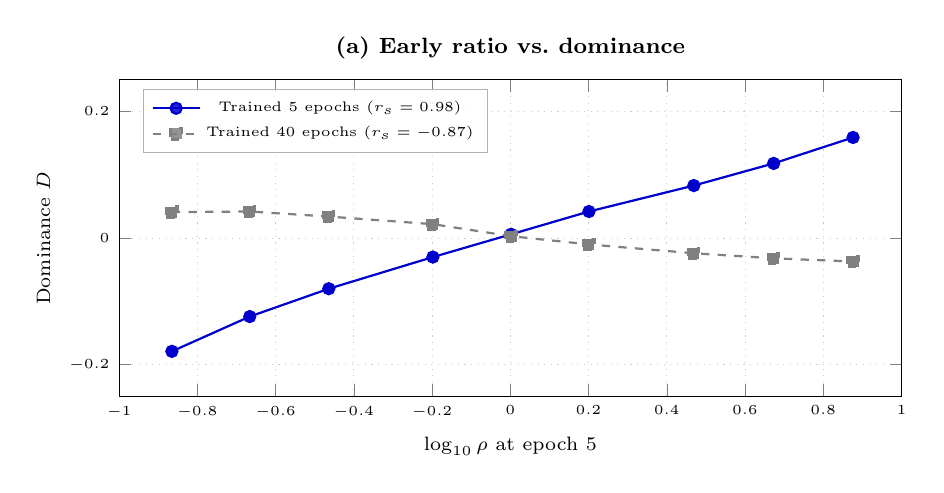
\begin{tikzpicture}
\begin{axis}[
    width=0.95\linewidth, height=5.6cm,
    title={(a) Early ratio vs.\ dominance},
    xlabel={$\log_{10}\rho$ at epoch 5}, ylabel={Dominance $D$},
    xmin=-1, xmax=1, ymin=-0.25, ymax=0.25,
    legend pos=north west,
]
% Mean of 5 seeds per input-scale ratio (0.05, 0.1, 0.2, 0.5, 1, 2, 5, 10, 20);
% x = mean log10(rho at epoch 5), y = test dominance Acc_A - Acc_V.
% Sources: results/processed/e2_causal_headroom_ep5_runs.csv (5 epochs), e2_causal_primary_runs.csv (40 epochs)
\addplot[blue!80!black, mark=*, thick] coordinates {(-0.865,-0.179)(-0.666,-0.124)(-0.464,-0.080)(-0.198,-0.030)(0.002,0.006)(0.201,0.042)(0.469,0.083)(0.673,0.118)(0.876,0.159)};
\addlegendentry{Trained 5 epochs ($r_s=0.98$)}
\addplot[gray, dashed, mark=square*, thick] coordinates {(-0.865,0.041)(-0.666,0.042)(-0.464,0.034)(-0.198,0.022)(0.002,0.003)(0.201,-0.010)(0.469,-0.024)(0.673,-0.032)(0.876,-0.037)};
\addlegendentry{Trained 40 epochs ($r_s=-0.87$)}
\end{axis}
\end{tikzpicture}
\end{minipage}\hfill
\begin{minipage}[t]{0.48\textwidth}
\centering
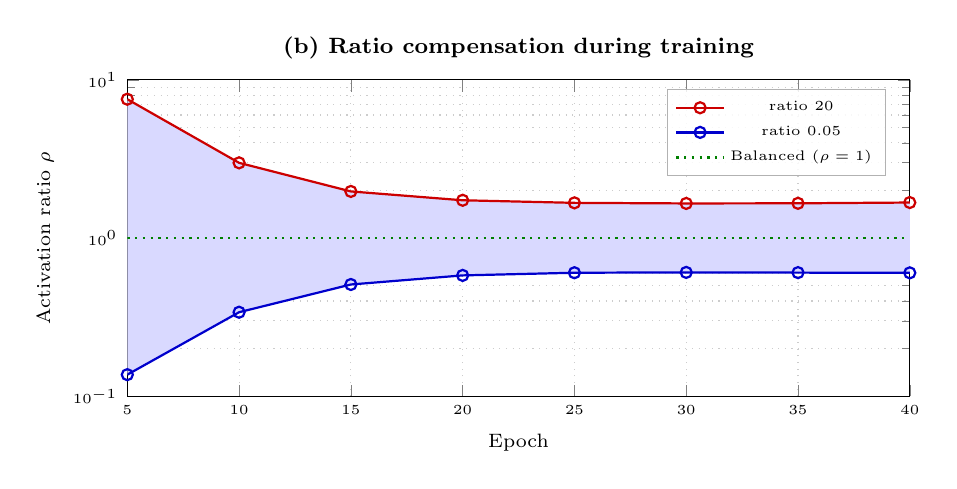
\begin{tikzpicture}
\begin{axis}[
    width=0.95\linewidth, height=5.6cm,
    title={(b) Ratio compensation during training},
    xlabel={Epoch}, ylabel={Activation ratio $\rho$},
    ymode=log, xmin=5, xmax=40, ymin=0.1, ymax=10,
    legend pos=north east,
]
% Mean activation ratio per epoch over 5 seeds (rho_history in results/raw/e2_causal/primary/run_r{20.0,0.05}_s*.json)
\addplot[name path=U, red!80!black, thick, mark=o] coordinates {(5,7.548)(10,2.990)(15,1.972)(20,1.734)(25,1.670)(30,1.656)(35,1.659)(40,1.678)};
\addlegendentry{ratio 20}
\addplot[name path=L, blue!80!black, thick, mark=o] coordinates {(5,0.137)(10,0.340)(15,0.509)(20,0.581)(25,0.604)(30,0.607)(35,0.605)(40,0.603)};
\addlegendentry{ratio 0.05}
\addplot[blue!15, forget plot] fill between[of=U and L];
\addplot[green!50!black, dotted, thick] coordinates {(5,1)(40,1)};
\addlegendentry{Balanced ($\rho=1$)}
\end{axis}
\end{tikzpicture}
\end{minipage}
\caption{(a) Activation ratio $\rho$ at epoch 5 vs.\ test dominance $D$ (mean of 5 seeds for each of 9 input-scale ratios): strongly rank-correlated after 5 epochs of training ($r_s = 0.98$), weak and reversed after 40 epochs ($r_s = -0.87$, $|D| < 0.05$). (b) Mean activation ratio per epoch for the two extreme input ratios: the span $[0.14, 7.55]$ at epoch 5 contracts to $[0.60, 1.68]$ by epoch 40 as the encoders adapt.}
\label{fig:early_diagnostic}
\end{figure*}

\subsection{RQ3: Optimizer Compensation Dynamics}
Table~\ref{tab:optimizer_updates} and Fig.~\ref{fig:optimizer_dynamics} compare Adam and SGD under gradient scaling ($\mathcal{T}_{\text{grad}}$, $\alpha = 100$).

\begin{table}[!t]
\centering
% Synthetic rows: results/phase1_decoupled/phase1_primary_seeds10.csv (gradient arm, 10 seeds, Student-t CIs).
% CREMA-D: results/cremad_disentangle/cremad_disentangle_primary.csv; divergence counts: results/phase3_cremad/phase3_cremad_scoped.csv
% and results/phase4_baselines/phase4_sgd_stable.csv.
\caption{Update and Gradient Ratios under Gradient Intervention ($\alpha = 100$); synthetic rows: Phase 1, 10 seeds, $\pm$ = Student-$t$ 95\% CI}
\label{tab:optimizer_updates}
\renewcommand{\arraystretch}{1.1}
\resizebox{\columnwidth}{!}{%
\begin{tabular}{lcc}
\toprule
\textbf{Metric} & \textbf{Adam} & \textbf{SGD} \\
\midrule
Gradient ratio $r_g$ (synthetic) & $100.6 \pm 1.3$ & $315.7 \pm 8.8$ \\
Update ratio $\rho_{\Delta\theta}$ (synthetic) & $1.001 \pm 0.011$ & $95.8 \pm 4.6$ \\
CREMA-D: $r_g \rightarrow \rho_{\Delta\theta}$ & $282.7 \rightarrow 1.61$ (baseline 1.65) & -- \\
Theory & cancellation & linear, $\sim\alpha$ \\
Diverged runs, synthetic & 0/80 & 0/80 \\
Diverged, CREMA-D, no clipping & 0/5 & fwd 3/5, grad 2/2 ($\eta = 3\times10^{-2}$); grad 5/5 ($\eta = 10^{-2}$) \\
Diverged, CREMA-D, clipping 1.0 & n/a & 0/5 per arm ($\eta = 10^{-2}$) \\
LR cancellation ($\eta_A = \eta/\alpha$) & n/a & $D = +0.003$ \\
\bottomrule
\end{tabular}}
\end{table}

% FIGURE 5 (two panels, full width)
\begin{figure*}[!t]
\centering
\begin{minipage}[t]{0.48\textwidth}
\centering
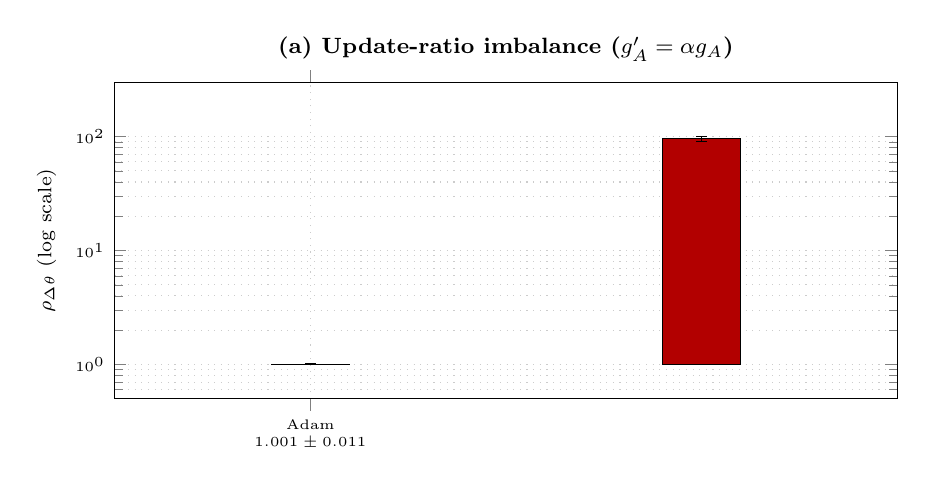
\begin{tikzpicture}
\begin{axis}[
    ybar, width=0.95\linewidth, height=5.6cm,
    title={(a) Update-ratio imbalance ($g_A' = \alpha g_A$)},
    symbolic x coords={adam,sgd}, xtick=data, enlarge x limits=0.5,
    xticklabels={{Adam\\$1.001\pm0.011$},{SGD\\$95.8\pm4.6$}},%
    x tick label style={align=center, font=\tiny},
    ymode=log, ymin=0.5, ymax=300, bar width=28pt,
    ylabel={$\rho_{\Delta\theta}$ (log scale)},
]
\addplot[bar shift=0pt, fill=blue!70!black, error bars/.cd, y dir=both, y explicit] coordinates {(adam,1.001) +- (0,0.011)};
\addplot[bar shift=0pt, fill=red!70!black, error bars/.cd, y dir=both, y explicit] coordinates {(sgd,95.8) +- (0,4.6)};
\end{axis}
\end{tikzpicture}
\end{minipage}\hfill
\begin{minipage}[t]{0.48\textwidth}
\centering
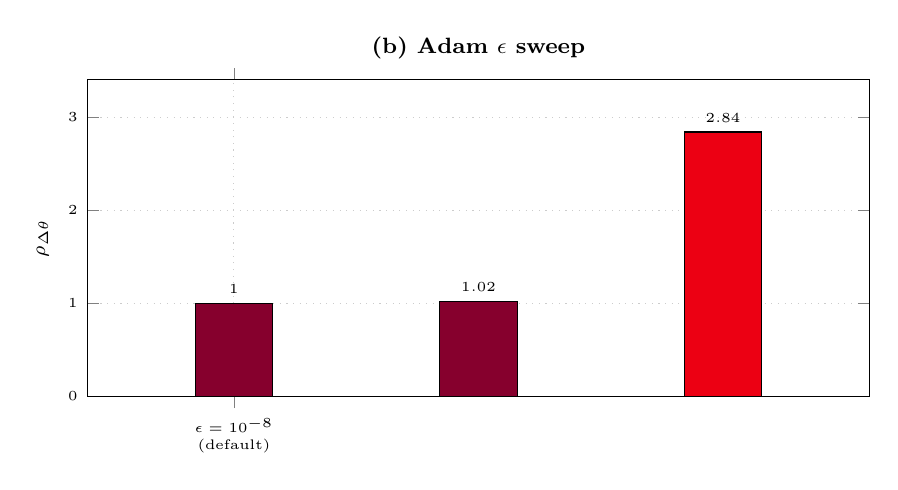
\begin{tikzpicture}
\begin{axis}[
    ybar, width=0.95\linewidth, height=5.6cm,
    title={(b) Adam $\epsilon$ sweep},
    symbolic x coords={e8,e4,e2}, xtick=data, enlarge x limits=0.3,
    xticklabels={{$\epsilon=10^{-8}$\\(default)},{$\epsilon=10^{-4}$},{$\epsilon=10^{-2}$\\(cancellation fails)}},
    x tick label style={align=center, font=\tiny},
    ymin=0, ymax=3.4, bar width=28pt,
    ylabel={$\rho_{\Delta\theta}$},
    nodes near coords, nodes near coords style={font=\tiny},
]
\addplot[bar shift=0pt, fill=purple!70!black] coordinates {(e8,1.00)};
\addplot[bar shift=0pt, fill=purple!70!black] coordinates {(e4,1.02)};
\addplot[bar shift=0pt, fill=red!70!purple] coordinates {(e2,2.84)};
\end{axis}
\end{tikzpicture}
\end{minipage}
\caption{(a) Update ratio $\rho_{\Delta\theta}$ under gradient scaling ($\alpha=100$): Adam cancels the scale almost perfectly while SGD drifts to $\approx\alpha$. (b) The cancellation breaks down as Adam's $\epsilon$ grows from $10^{-8}$ to $10^{-2}$.}
\label{fig:optimizer_dynamics}
\end{figure*}

\textbf{1) Adaptive cancellation in Adam.} As predicted by Eq.~\eqref{eq:adam_cancellation}, Adam yields $\rho_{\Delta\theta}^{(\text{Adam})} = 1.001 \pm 0.011$: the multiplier $\alpha$ is absorbed by the running second-moment buffer, leaving parameter trajectories invariant to gradient magnitude.

\textbf{2) Drift in SGD.} SGD yields $\rho_{\Delta\theta}^{(\text{SGD})} = 95.8 \pm 4.6$, close to the injected $\alpha = 100$. On CREMA-D without clipping this destabilizes optimization: at $\eta = 3\times10^{-2}$, 3 of 5 forward seeds and both gradient seeds that were run diverged, and the two surviving forward seeds fell to near-chance validation accuracy (0.171). Global gradient-norm clipping (max-norm 1.0, $\eta = 10^{-2}$) removes the divergence (0 of 5 gradient seeds, versus 5 of 5 without clipping) and leaves the per-modality gradient ratio unchanged (1011.3 before and after clipping).

\textbf{3) Learning-rate cancellation.} In Phase 2 (Finding 4), scaling the learning rate of modality $A$ by $\eta_A = \eta/\alpha$ returns the update ratio to $0.99$ and dominance to $D = +0.003$, matching the unperturbed baseline.

\textbf{4) Breakdown under $\epsilon$ sweeps.} In Phase 2 (Finding 3), sweeping $\epsilon \in \{10^{-8}, 10^{-4}, 10^{-2}\}$ shifts $\rho_{\Delta\theta}$ from $1.00$ to $1.02$ to $2.84$ (Fig.~\ref{fig:optimizer_dynamics}(b)). When $\epsilon$ approaches the gradient magnitude, adaptive scaling degrades toward SGD-like behavior.

\subsection{RQ4: CREMA-D Validation and the Masking Illusion}
Table~\ref{tab:crema_results} and Fig.~\ref{fig:cremad_decoupled} give the Phase 3 results on CREMA-D (5 seeds, AdamW).

\begin{table}[!t]
\centering
\caption{CREMA-D: Naive Zero-Masking vs.\ Decoupled Metrics (AdamW, 5 seeds)}
\label{tab:crema_results}
\renewcommand{\arraystretch}{1.1}
\resizebox{\columnwidth}{!}{%
\begin{tabular}{lcc}
\toprule
% Paired Student-t 95% CIs, n = 5 (t_{0.975,4} = 2.776), from results/phase2_mechanism/phase2_cremad_probe.csv (p: 8e-5, 0.28, 0.23, 0.022)
\textbf{Metric} & \textbf{Shift ($\pm$ 95\% CI)} & \textbf{Status} \\
\midrule
Naive masked dominance ($\Delta D_{\text{mask}}$) & $+0.259 \pm 0.044$ & significant ($p<0.01$) \\
Mean-ablation dominance & $+0.012 \pm 0.027$ & n.s.\ ($p>0.05$) \\
Shapley contribution ($\Delta\phi_A$) & $+0.014 \pm 0.026$ & n.s.\ ($p>0.05$) \\
Frozen linear probe accuracy & $+0.023 \pm 0.017$ & intact \\
\bottomrule
\end{tabular}}
\end{table}

\begin{figure}[!t]
\centering
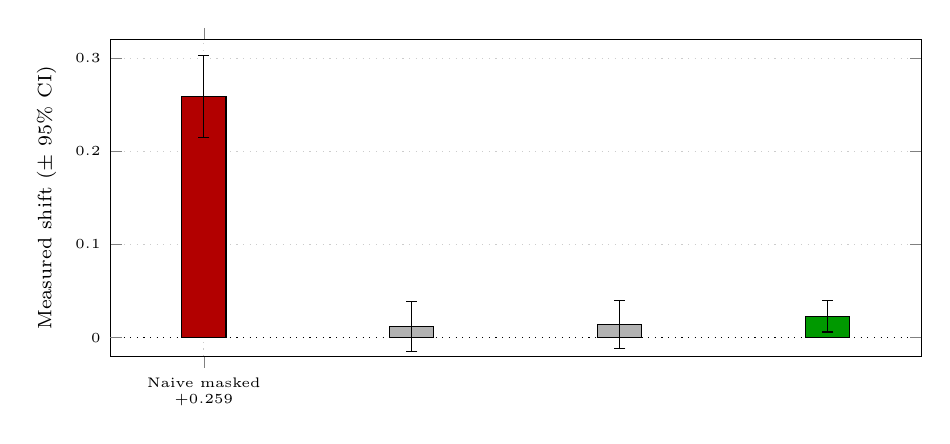
\begin{tikzpicture}
\begin{axis}[
    ybar, width=0.98\columnwidth, height=5.6cm,
    symbolic x coords={m,a,s,p}, xtick=data, enlarge x limits=0.15,
    xticklabels={{Naive masked\\$+0.259$},{Mean ablation\\$+0.012$},{Shapley $\Delta\phi_A$\\$+0.014$},{Frozen probe\\$+0.023$}},
    x tick label style={align=center, font=\tiny},
    bar width=16pt, ymin=-0.02, ymax=0.32,
    ylabel={Measured shift ($\pm$ 95\% CI)},%
    extra y ticks=0, extra y tick labels={}, extra y tick style={grid=major, grid style={black, thin}},
]
\addplot[bar shift=0pt, fill=red!70!black, error bars/.cd, y dir=both, y explicit] coordinates {(m,0.259) +- (0,0.044)};
\addplot[bar shift=0pt, fill=gray!60, error bars/.cd, y dir=both, y explicit] coordinates {(a,0.012) +- (0,0.027)};
\addplot[bar shift=0pt, fill=gray!60, error bars/.cd, y dir=both, y explicit] coordinates {(s,0.014) +- (0,0.026)};
\addplot[bar shift=0pt, fill=green!60!black, error bars/.cd, y dir=both, y explicit] coordinates {(p,0.023) +- (0,0.017)};
\end{axis}
\end{tikzpicture}
\caption{CREMA-D: naive zero-masking vs.\ decoupled metrics (Finding W2). The large dominance under masking ($+0.259$) is not reproduced by mean ablation ($+0.012$), Shapley analysis ($+0.014$), or probes ($+0.023$), consistent with a classifier out-of-distribution artifact.}
\label{fig:cremad_decoupled}
\end{figure}

This yields \textbf{Finding W2}:
\begin{itemize}
    \item Under zero-masking, the forward intervention shows strong dominance: $\Delta D_{\text{mask}} = +0.259 \pm 0.044$ ($p < 0.01$). Prior practice would read this as evidence that scale causes real-world collapse.
    \item Under mean ablation the shift falls to $+0.012 \pm 0.027$ ($p > 0.05$).
    \item Under Shapley contribution it is $+0.014 \pm 0.026$ ($p > 0.05$).
    \item Under frozen linear probes, modality-$A$ accuracy is unimpaired ($\Delta \text{Acc}_{\text{probe}} = +0.023 \pm 0.017$).
\end{itemize}
This discrepancy indicates that, on this real-world data, the apparent collapse detected by zero-masking is largely an artifact of classifier-head covariate shift, while the encoder representations remain discriminative.
The same dissociation appears with stabilized SGD (Phase 4, clipping 1.0): the gradient intervention moves masked dominance by $+0.200 \pm 0.050$, while mean ablation ($-0.001$), Shapley ($+0.002$) and the audio probe ($-0.001$) do not change.

% -----------------------------------------------------------------------------
% VII. ERROR ANALYSIS
% -----------------------------------------------------------------------------
\section{Error Analysis and Failure Modes}

\subsection{Classifier-Head Covariate Shift under Zero-Masking}
Consider the fusion pre-activation $z = W_f [h_A; h_V]$. Trained under forward scaling $\alpha = 100$, the linear head weights adapt to the numerical disparity such that $W_{f, A} \approx \frac{1}{\alpha} W_{f, A}^{(0)}$ while $W_{f, V} \approx W_{f, V}^{(0)}$. Consequently, setting $h_A \leftarrow \mathbf{0}$ shifts the fusion pre-activation by $\Delta z \approx - W_{f, A} (\alpha h_A) \approx - W_{f, A}^{(0)} h_A$, whereas masking $h_V \leftarrow \mathbf{0}$ shifts it by $\Delta z \approx - W_{f, V}^{(0)} h_V$. Because the head has adapted to the numerical disparity during joint training, clamping an input channel to zero abruptly displaces the pre-activation far outside the learned distribution manifold, generating severe classification degradation that reflects classifier-head covariate shift rather than underlying encoder feature erosion.

\subsection{Optimization Instability in Non-Adaptive Regimes}
A second failure mode arises when scale interventions are used with SGD without per-modality learning-rate matching. %
On CREMA-D, at $\eta = 3\times10^{-2}$ without clipping, SGD training diverged (non-finite loss) in 60\% of forward runs and 100\% of gradient runs. Global gradient-norm clipping at 1.0 removed every divergence (0 of 5 runs per arm) without changing the per-modality gradient ratio. Gradient-modulation strategies such as OGM-GE may therefore be unstable with non-adaptive optimizers unless paired with gradient clipping.

% -----------------------------------------------------------------------------
% VIII. DISCUSSION
% -----------------------------------------------------------------------------
\section{Discussion and Practical Guidelines}

\subsection{Why Feature Scale Does Not Explain Real-World Collapse}
Across both benchmarks the scale hypothesis has a clear boundary. In low-capacity synthetic models, extreme forward scale distorts early optimization enough to degrade encoder representations ($\Delta \text{Probe} = -0.0339$). %
On CREMA-D, with small CNN encoders trained from scratch, the audio encoder is already close to its own ceiling (frozen audio probe 0.522 at baseline), so there is little headroom for its representation to change, while the head's calibration to the scaled input makes zero-masking very damaging. We therefore suggest looking beyond numerical scale---toward semantic redundancy, gradient conflict, and regularization disparities---to explain real-world collapse. Because this conclusion rests on a single real dataset, it should be read as evidence rather than proof.

\subsection{Prescriptive Guidelines for Multimodal Evaluation}
We propose three evaluation standards:
\begin{enumerate}
    \item \textbf{Do not use zero-masking in isolation} to claim modality dominance.
    \item \textbf{Report decoupled probes:} when suppression is asserted, report linear probes trained on frozen representations.
    \item \textbf{Report cooperative contribution metrics:} mean ablation and Shapley values should accompany accuracy-based dominance measures.
\end{enumerate}

% -----------------------------------------------------------------------------
% IX. LIMITATIONS
% -----------------------------------------------------------------------------
\section{Limitations and Future Work}
\begin{itemize}
    \item Due to compute and disk space constraints (RTX 4070, 8.6 GB VRAM, 53 GB disk), the evaluation of real world material is limited here to CREMA-D, and Kinetics-Sounds, AVE and VGGSound should be run on larger clusters.
    \item Without clipping, SGD at extreme scale diverged in most CREMA-D runs; the clipped runs (Phase 4) are stable but rest on 5 seeds, so the SGD results on real data should be read as preliminary.
    \item We investigate small CNN backbones trained end-to-end from scratch; applying scale interventions to pre-trained multimodal transformers (e.g., CLIP, Flamingo) is a crucial next step.
\end{itemize}

% -----------------------------------------------------------------------------
% X. REPRODUCIBILITY
% -----------------------------------------------------------------------------
\section{Reproducibility Statement}
All configurations (e.g.\ \texttt{configs/boundary.yaml} for the synthetic phases and \texttt{configs/cremad.yaml} for CREMA-D) and all seeds ($n=10$ synthetic, $n=5$ real) are version-controlled in git commit \texttt{c76c5e6} along with environment specifications and analysis scripts. Before running the trial, passed unit and regression tests (12/12). Implementations of metrics, routines for training probes, and synthetic data generators are provided along with the codebase.

% -----------------------------------------------------------------------------
% XI. CONCLUSION
% -----------------------------------------------------------------------------
\section{Conclusion}
We examined if there was a feature-magnitude disparity between the modality encoders that led to modality collapse. %
We showed that (1) the early activation-norm ratio tracks early dominance ($r_s = 0.98$ at epoch 5) but does not predict converged dominance, because trainable encoders compensate for the scale; (2) Adam's adaptive moments correct for scale differences in the gradients, while SGD suffers from extreme update drift; and (3) when using frozen probes, mean ablation and Shapley values, extreme forward scaling is indeed a degradation of the representation on low-capacity synthetic models, but not supported by either of these metrics on real audio-visual data, and showing consistency with the covariate shift phenomenon of classifier-heads. We encourage the community to use a decoupled evaluation protocol and be careful with scale-based explanations of modality collapse.

% -----------------------------------------------------------------------------
% REFERENCES
% -----------------------------------------------------------------------------
\begin{thebibliography}{00}

\bibitem{wang2020makes}
W. Wang, D. Tran, and M. Feiszli, ``What makes training multi-modal classification networks hard?'' in \emph{Proc. IEEE/CVF Conf. Comput. Vis. Pattern Recognit. (CVPR)}, 2020, pp. 12695--12705.

\bibitem{peng2022balanced}
X. Peng, Y. Wei, A. Deng, D. Wang, and D. Hu, ``Balanced multimodal learning via on-the-fly gradient modulation,'' in \emph{Proc. IEEE/CVF Conf. Comput. Vis. Pattern Recognit. (CVPR)}, 2022, pp. 8238--8247.

\bibitem{fan2023pmr}
Y. Fan, W. Xu, H. Wang, J. Wang, and S. Guo, ``PMR: Prototypical modal rebalance for multimodal learning,'' in \emph{Proc. IEEE/CVF Conf. Comput. Vis. Pattern Recognit. (CVPR)}, 2023, pp. 20029--20038.

\bibitem{wu2022characterizing}
N. Wu, S. Jastrzebski, K. Cho, and K. J. Geras, ``Characterizing and overcoming the greedy nature of learning in multi-modal deep neural networks,'' in \emph{Proc. Int. Conf. Mach. Learn. (ICML)}, 2022, pp. 24043--24055.

\bibitem{baltrusaitis2019multimodal}
T. Baltru\v{s}aitis, C. Ahuja, and L.-P. Morency, ``Multimodal machine learning: A survey and taxonomy,'' in \emph{IEEE Trans. Pattern Anal. Mach. Intell.}, vol. 41, no. 2, pp. 423--443, 2019.

\bibitem{cao2014crema}
H. Cao, D. G. Cooper, M. K. Keutmann, R. C. Gur, A. Nenkova, and R. Verma, ``CREMA-D: Crowd-sourced emotional multimodal actors dataset,'' \emph{IEEE Trans. Affect. Comput.}, vol. 5, no. 4, pp. 377--390, 2014.

\bibitem{alain2016understanding}
G. Alain and Y. Bengio, ``Understanding intermediate layers using linear classifier probes,'' in \emph{Proc. ICLR Workshop}, 2017.

\bibitem{lundberg2017unified}
S. M. Lundberg and S.-I. Lee, ``A unified approach to interpreting model predictions,'' in \emph{Adv. Neural Inf. Process. Syst. (NeurIPS)}, vol. 30, 2017, pp. 4765--4774.
\bibitem{shapley1953value}
L. S. Shapley, ``A value for n-person games,'' in \emph{Contributions to the Theory of Games}, vol. 2, 1953, pp. 307--317.
\bibitem{morcos2018importance}
A. S. Morcos, D. G. T. Barrett, N. C. Rabinowitz, and M. Botvinick, ``On the importance of single directions for generalization,'' in \emph{Proc. ICLR}, 2018.
\bibitem{kingma2015adam}
D. P. Kingma and J. Ba, ``Adam: A method for stochastic optimization,'' in \emph{Proc. ICLR}, 2015.
\bibitem{loshchilov2019decoupled}
I. Loshchilov and F. Hutter, ``Decoupled weight decay regularization,'' in \emph{Proc. ICLR}, 2019.
\bibitem{wilson2017marginal}
A. C. Wilson, R. Roelofs, M. Stern, N. Srebro, and B. Recht, ``The marginal value of adaptive gradient methods in machine learning,'' in \emph{Adv. Neural Inf. Process. Syst. (NeurIPS)}, vol. 30, 2017, pp. 4148--4158.
\bibitem{zhang2020adaptive}
J. Zhang et al., ``Why are adaptive methods good for attention models?,'' in \emph{Adv. Neural Inf. Process. Syst. (NeurIPS)}, vol. 33, 2020, pp. 15383--15393.
\bibitem{ba2016layer}
J. L. Ba, J. R. Kiros, and G. E. Hinton, ``Layer normalization,'' arXiv:1607.06450, 2016.
\end{thebibliography}
\end{document}